\section{\glsentrylongpl{cfa} and Formal Languages}\label{sec:cfa-languages}

\glspl{fa} stand at the very origin of algorithmic language processing and they form the canonical recognisers of the \glspl{reg}, a class originally isolated by Kleene through rational expressions \cite{kleene1951representationof}. Their mathematical roots trace back to Chomsky's hierarchy of grammars \cite{chomsky1959certain} and to the seminal definition of machine based language recognition given independently by Rabin and Scott \cite{rabin1959finite}. The structural essence of regularity was soon clarified by the Myhill and Nerode equivalence relation, which provides a necessary and sufficient criterion for finite recognisability without reference to a particular device \cite{myhill1957finite,nerode1958linear}. These results, later unified in modern textbooks \cite{hopcroft2001introduction,aho1974design,sipser1996introduction}, still underpin today's compiler front-ends, hardware verification workflows and network protocol design.

Historically four computational patterns crystallised out of the study of \glspl{cfa}. The first is the \gls{dfa}, a fully deterministic device that admits a single computation path and thus offers linear time membership testing together with minimal state equivalence \cite{hopcroft2001introduction}. The second is the \gls{nfa}, which explores many futures in parallel and enjoys an exponential succinctness advantage while remaining equivalent in expressive power to the deterministic model \cite{rabin1959finite}. Probabilistic branching leads to the \gls{pfa}, an automaton that attaches transition weights and decides membership relative to a rational cut point; with an isolated threshold it still recognises only \glspl{reg} \cite{paz2014introduction} whereas an arbitrary threshold allows stochastic languages that are not regular \cite{turakainen1969generalized}. Finally lifting the read head restriction yields two-way variants that may revisit earlier symbols and thereby capture algorithms such as lexical scanners with look ahead, yet they do not surpass regular expressiveness \cite{freivalds1981probabilistic}.

This section surveys the algebraic landscape in which these machines operate. It begins with precise notions of words, grammars and closure properties, establishing the equivalence between regular grammars, rational expressions and \glspl{cfa}. It then presents the four concrete models just outlined, emphasising historical context, formal properties such as closure and minimisation, and illustrative examples that will serve as running motifs throughout the thesis. Together these elements motivate later chapters, where classical finite-memory computation is extended first to probabilistic and finally to quantum domains.

\subsection{Languages, Grammars and Regularity}\label{subsec:foundations}

The study of \glspl{cfa} rests on an algebraic view of words.  
Starting from finite alphabets, we assemble strings through concatenation,  
obtain the free monoid $\Sigma^{\ast}$,  
and finally analyse those subsets of $\Sigma^{\ast}$ that arise in computation.  
This section revisits the classical path from atomic symbols to the full power of regular grammars.  
Along the way the narrative highlights why each construction matters later for deterministic, nondeterministic and probabilistic machines.  

\begin{definition}[Alphabet]\label{def:alphabet}
A non empty finite set $\Sigma$ of symbols is called an alphabet \cite{hopcroft2001introduction}.  
\end{definition}

Finite alphabets formalise the intuitive notion of a computer input device that produces a bounded repertoire of symbols.  
Restricting to finite $\Sigma$ is essential for decidability results that follow in the automata hierarchy.  

\begin{definition}[String and Concatenation]\label{def:string}
A string, or word, over $\Sigma$ is a finite sequence
$w=a_{1}a_{2}\dots a_{n}$ with $a_{i}\in\Sigma$.  
The empty word is denoted $\varepsilon$.  
Concatenation $u\cdot v$ appends the sequence of $v$ to $u$ \cite{hopcroft2001introduction}.  
\end{definition}

Concatenation is associative, admits $\varepsilon$ as identity and thus endows  
the set of words with a monoid structure.  
This algebraic property underpins many closure proofs for language classes.  

\begin{notation}
The set of all words over $\Sigma$ forms the free monoid
$\Sigma^{\ast}$ under concatenation with identity $\varepsilon$ \cite{hopcroft2001introduction}.  
\end{notation}

\begin{definition}[Formal Language]\label{def:language}
Any subset $L\subseteq\Sigma^{\ast}$ is a language \cite{hopcroft2001introduction}.  
\end{definition}

Automata theory evaluates the descriptive cost of specifying $L$.  
The smaller the machine needed to decide membership, the simpler the language is deemed.  

\begin{concept}[Regular Grammar]\label{concept:regular-grammar}
A type~3 grammar in Chomsky's hierarchy~\ref{fig:chomsky-hierarchy} generates the \glspl{reg} \cite{chomsky1959certain}.  
\end{concept}

\begin{figure}[h]
  \centering
  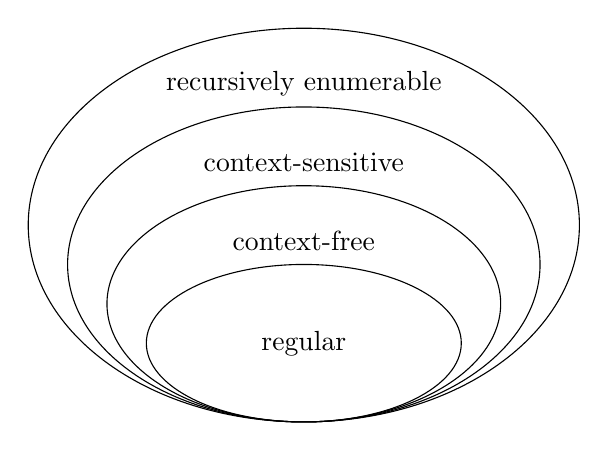
\begin{tikzpicture}
      %TODO: add colours to ellipses without overlapping
      \draw (0,0) ellipse (2 and 1);
      \draw (0,0.5) ellipse (2.5 and 1.5);
      \draw (0,1) ellipse (3 and 2);
      \draw (0,1.5) ellipse (3.5 and 2.5);
      \node at (0,0) {regular};
      \node at (0,1.3) {context-free};
      \node at (0,2.3) {context-sensitive};
      \node at (0,3.3) {recursively enumerable};
  \end{tikzpicture}
  \caption{Chomsky hierarchy of formal languages}
  \label{fig:chomsky-hierarchy}
\end{figure}


Type~3 productions constrain derivations to one non terminal symbol at most,  
ensuring finite memory during parsing.  
The resulting languages coincide with those accepted by finite automata, an insight traced back to Kleene.  

\begin{theorem}[Kleene Correspondence]\label{thm:kleene}
The following families coincide:
\begin{enumerate}
  \item languages generated by type~3 grammars,
  \item languages denoted by regular expressions,
  \item languages recognised by \glspl{cfa}.
\end{enumerate}
\cite{kleene1951representationof}
\end{theorem}

Kleene's theorem supplies three interchangeable viewpoints:  
syntactic derivation, algebraic expression and operational recognition.  
Switching among them allows proofs to borrow the strengths of each representation,  
for instance when optimising a \gls{dfa} derived from a regular expression.  

\begin{proposition}[Closure of \glspl{reg}]\label{prop:closure}
Let ${\cal R}$ denote the class of \glspl{reg}.  
If $L_{1},L_{2}\in{\cal R}$ then so are
$L_{1}\cup L_{2}$, $L_{1}\cap L_{2}$, $\overline{L_{1}}$,
$L_{1}\,L_{2}$ and $L_{1}^{\ast}$ \cite{hopcroft2001introduction}.  
\end{proposition}

Closure under Boolean operations follows directly from set algebra on \gls{dfa} state sets,  
while closure under concatenation and star is established with product and power set constructions.  
These properties justify the pervasive role of \glspl{reg} in software tools:  
complex lexical patterns can be decomposed, manipulated and recombined without leaving ${\cal R}$.  

\begin{theorem}[Myhill-Nerode]\label{thm:myhill-nerode}
A language $L\subseteq\Sigma^{\ast}$ is regular  
iff the relation
$x\equiv_{L}y \;\Longleftrightarrow\; \forall z\in\Sigma^{\ast}\colon  
xz\in L \;\Leftrightarrow\; yz\in L$
admits finitely many equivalence classes \cite{hopcroft2001introduction}.  
\end{theorem}

The theorem supplies a minimality criterion:  
the number of equivalence classes equals the state count of the smallest \gls{dfa} for $L$.  
In compiler construction this bound translates into memory requirements for lexical analysers.  

\begin{example}[Simple \gls{reg}]\label{ex:reg-lang}
For $\Sigma=\{0,1\}$ the set
$L=\{w\in\Sigma^{\ast}\mid w\text{ ends in }1\}$ is regular because it
is described by the regular expression $\Sigma^{\ast}1$ \cite{hopcroft2001introduction}.  
\end{example}

The language of Example~\ref{ex:reg-lang} illustrates how a single positional constraint  
is captured by a two-state \gls{dfa}, matching the Myhill-Nerode bound.  

\begin{observation}\label{obs:why-regular-matters}
\glspl{reg} admit linear time membership tests and deterministic
finite-state representations; therefore they are widely used in lexical
tokenisers, model checking and hardware controllers \cite{aho1974design}.  
\end{observation}

In summary, regularity offers a balance between expressive adequacy for many practical patterns  
and tractable analysis, providing the theoretical bedrock on which later subsections build deterministic,  
nondeterministic and quantum extensions of the finite automaton paradigm.

\subsection{Deterministic Finite Automaton}\label{subsec:dfa}

Among abstract machines the \gls{dfa} offers the most transparent model
of computation.  From any configuration the current state and the symbol
under the input head select exactly one successor state
\cite{hopcroft2001introduction}.  This functional behaviour yields predictable
memory usage, permits direct hardware realisation and supports efficient
software simulation.

\begin{definition}[Deterministic Finite Automaton]\label{def:dfa}
A \gls{dfa} is a quintuple
$M=(Q,\Sigma,\delta,q_{0},F)$ where
$Q$ is a finite set of states,
$\Sigma$ is an input alphabet,
$\delta\colon Q{\times}\Sigma\to Q$ is the transition map,
$q_{0}\in Q$ is the start state and
$F\subseteq Q$ is the set of accepting states
\cite{hopcroft2001introduction}.
\end{definition}

For analysis it is convenient to lift $\delta$ to words.  The extended
map $\hat{\delta}\colon Q{\times}\Sigma^{\ast}\to Q$ satisfies
$\hat{\delta}(q,\varepsilon)=q$ and
$\hat{\delta}(q,aw)=\hat{\delta}(\delta(q,a),w)$.  Structural induction
on the length of $w$ shows that $\hat{\delta}$ is total and unique
\cite{hopcroft2001introduction}.

\begin{proposition}[Unique computation path]\label{prop:dfa-path}
For every input word $w\in\Sigma^{\ast}$ the sequence
$\,q_{0},
\hat{\delta}(q_{0},a_{1}),
\hat{\delta}(q_{0},a_{1}a_{2}),
\dots,
\hat{\delta}(q_{0},w)\,$
is the only path in $M$ labelled by $w$
\cite{hopcroft2001introduction}.
\end{proposition}

\begin{definition}[Accepted language]\label{def:dfa-lang}
The language recognised by $M$ is
$L(M)=\{\,w\in\Sigma^{\ast}\mid \hat{\delta}(q_{0},w)\in F\,\}$
\cite{hopcroft2001introduction}.
\end{definition}

Finite automata gain analytic power from the right invariant congruence
\[x\equiv_{L}y \Longleftrightarrow
  \forall z\in\Sigma^{\ast}\colon
  xz\in L \Leftrightarrow yz\in L.\]

\begin{theorem}[Myhill Nerode]\label{thm:mn-dfa}
A language $L\subseteq\Sigma^{\ast}$ is regular
iff the relation $\equiv_{L}$ has finitely many equivalence classes
\cite{nerode1958linear}.
\end{theorem}

The number of classes equals the size of the smallest \gls{dfa} for $L$,
so state minimisation amounts to quotienting by $\equiv_{L}$.

\begin{theorem}[DFA minimisation]\label{thm:minimisation}
Every \gls{dfa} $M$ possesses a unique minimal
equivalent \gls{dfa} $M_{\mathrm{min}}$ up to isomorphism
\cite{moore1956gedanken}. The Hopcroft partition refinement algorithm computes
$M_{\mathrm{min}}$ in $O(|Q|\log|Q|)$ time \cite{hopcroft1971n}.
\end{theorem}

Because a \gls{dfa} is finite, many questions are decidable.

\begin{proposition}[Algorithmic questions]\label{prop:dfa-decision}
Given \glspl{dfa} $M_{1},M_{2}$ over $\Sigma$ one can decide in
polynomial time: emptiness of $L(M_{1})$, finiteness of $L(M_{1})$,
equivalence $L(M_{1})=L(M_{2})$ and inclusion
$L(M_{1})\subseteq L(M_{2})$ \cite{hopcroft2001introduction}.
\end{proposition}

\begin{example}[Even number of \(a\) symbols]\label{ex:dfa-even}
Figure~\ref{fig:dfa-even-a} depicts the \gls{dfa} recognising
$L=\{\,w\in\{a,b\}^{\ast}\mid
       \text{the number of }a\text{ symbols is even}\,\}$
\cite{hopcroft2001introduction}.  The relation $\equiv_{L}$ has exactly two
classes, matching the two states shown.
\end{example}

\begin{figure}[H]
    \centering
    \begin{tikzpicture}[->,>=stealth,node distance=30mm]
      \node[state,initial,accepting] (qe) {$q_{\mathrm{even}}$};
      \node[state]                   (qo) [right of=qe] {$q_{\mathrm{odd}}$};
      \path (qe) edge[loop above] node {$b$} (qe)
            (qo) edge[loop above] node {$b$} (qo)
            (qe) edge[bend left, sloped, above]  node {$a$} (qo)
            (qo) edge[bend left, sloped, above]  node {$a$} (qe);
    \end{tikzpicture}
    \caption{\gls{dfa} for words with an even number of \(a\) symbols
    \cite{hopcroft2001introduction}.}
    \label{fig:dfa-even-a}
\end{figure}

\begin{example}[Binary multiples of three]\label{ex:dfa-mult3}
Over $\Sigma=\{0,1\}$ the set
$L=\{\,w\mid w\text{ interpreted as binary represents a multiple of }3\,\}$
is regular.  A machine with three states tracks the remainder modulo
three after each bit is read \cite{sipser1996introduction}.
\end{example}

\glspl{dfa} support linear time scanning with constant memory.
Compilers use them for lexical analysis, hardware circuits translate
transitions into flip flops, and many regular expression engines adopt
deterministic evaluation to guarantee predictable performance
\cite{aho1974design}.  Deterministic automata thus form the
baseline against which later sections measure the expressive gains and
computational costs of nondeterministic, weighted and quantum variants.

\subsection{Nondeterministic Finite Automaton}\label{subsec:nfa}

Where a \gls{dfa} follows a single computation path, a \gls{nfa} may
branch whenever several successor states are permitted.  The branching
semantics can reduce the number of states that must be stored
explicitly, but it transfers complexity to the acceptance relation
\cite{rabin1959finite}.

\begin{definition}[Nondeterministic Finite Automaton]\label{def:nfa}
A \gls{nfa} is a quintuple
$M=(Q,\Sigma,\delta,q_{0},F)$ with
finite-state set $Q$, input alphabet $\Sigma$, transition map
$\delta\colon Q{\times}\Sigma_{\varepsilon}\to\mathcal{P}(Q)$,
start state $q_{0}\in Q$ and set of final states $F\subseteq Q$.
Here $\Sigma_{\varepsilon}=\Sigma\cup\{\varepsilon\}$ adjoins the empty
word to allow silent moves \cite{rabin1959finite}.
\end{definition}

Extending $\delta$ to words first requires the
$\varepsilon$-closure operator
$\operatorname{E}(S)=
  \bigl\{\,q\in Q\mid
          \exists p\in S\colon
          p\xrightarrow{\varepsilon^{\ast}} q\,\bigr\}$

For $w=a_{1}a_{2}\dots a_{n}$ define recursively  
$S_{0}=\operatorname{E}\bigl(\{q_{0}\}\bigr)$ and  
$S_{i+1}=  
\operatorname{E}\bigl(\,\bigcup_{q\in S_{i}}\delta(q,a_{i+1})\bigr)$.
The set $S_{n}$ collects every state reachable after reading $w$.

\begin{lemma}[Acceptance criterion]\label{lem:nfa-accept}
The automaton $M$ accepts $w$ exactly when
$S_{|w|}\cap F\neq\emptyset$ \cite{hopcroft2001introduction}.
\end{lemma}

Nondeterminism does not enlarge expressive power.

\begin{theorem}[Subset construction]\label{thm:subset}
For an \gls{nfa} with $n$ states the powerset construction produces an
equivalent \gls{dfa} whose state set has size at most $2^{n}$
\cite{rabin1959finite}.  
\end{theorem}

Silent moves can be eliminated first; the combined transformation
preserves language and produces a \gls{dfa} whose transition map
operates on subsets of $Q$.

\begin{proposition}[Elimination of $\varepsilon$ transitions]\label{prop:eps-removal}
An \gls{nfa} with $\varepsilon$ moves has an equivalent
$\varepsilon$-free \gls{nfa} with the same number of states
\cite{hopcroft2001introduction}.
\end{proposition}

Although determinisation may yield an exponential blow-up, the reverse
direction is more benign.

\begin{observation}[Succinctness gap]\label{obs:nfa-size}
There exist languages $L_{n}\subseteq\Sigma^{\ast}$ whose minimal
\gls{nfa} requires $\Theta(n)$ states while every equivalent
\gls{dfa} needs $\Theta(2^{n})$ states
\cite{aho1974design}.
\end{observation}

The gap justifies the preference for \glspl{nfa} as intermediate
representations in regular expression engines that ultimately generate a
\gls{dfa} only for performance critical fragments.

\begin{example}[Words of length one]\label{ex:nfa-length1}
Figure~\ref{fig:nfa-figure} shows a four state \gls{nfa} that accepts
$\Sigma^{1}$.  Two silent moves branch from $q_{0}$; each branch consumes
one symbol then moves to the final state $q_{f}$
\cite{rabin1959finite}.
\end{example}

\begin{figure}[H]
    \centering
    \begin{tikzpicture}[->,>=stealth,node distance=11mm,auto]
      \node[state,initial] (q0) {$q_{0}$};
      \node[state]         (q1) [above right=of q0] {$q_{1}$};
      \node[state]         (q2) [below right=of q0] {$q_{2}$};
      \node[state,accepting] (qf) [right=of q1] {$q_{f}$};
      %
      \path (q0) edge[bend left]  node {$\varepsilon$} (q1)
            (q0) edge[bend right] node[swap] {$\varepsilon$} (q2)
            (q1) edge node {$\Sigma$} (qf)
            (q2) edge node[swap] {$\Sigma$} (qf);
    \end{tikzpicture}
    \caption{\gls{nfa} for all words whose length equals one
             \cite{rabin1959finite}.}
    \label{fig:nfa-figure}
\end{figure}

Decision problems for \glspl{nfa} inherit tractability from their
deterministic counterparts because determinisation is constructive;
emptiness, finiteness and equivalence remain decidable in polynomial
time with respect to the size of the generated \gls{dfa}
\cite{hopcroft2001introduction}.  Subsequent sections compare these classical
results with the complexity landscape of probabilistic and quantum
extensions.

\subsection{Probabilistic Finite Automaton}\label{subsec:pfa}

\glspl{cfa} represent discrete control without any source
of uncertainty.  By attaching probabilities to transitions we obtain a
model that evolves like a Markov chain driven by the scanned word.
These \glspl{pfa} form the finite-memory analogue of probabilistic
Turing machines and supply the algebraic core of hidden Markov models
\cite{rabin1963probabilistic}.

\begin{definition}[Probabilistic Finite Automaton]\label{def:pfa}
  A \gls{pfa} is a quintuple
  \[
    M=(Q,\Sigma,\{\delta(a)\}_{a\in\Sigma},\mathbf{i},F)
  \]
  where
  \begin{itemize}
    \item $Q$ is a finite-state set,
    \item $\Sigma$ is an input alphabet,
    \item for every $a\in\Sigma$ the matrix
          $\delta(a)\in[0,1]^{Q\times Q}$ is
          row-stochastic, that is
          $\sum_{q'\in Q}\delta(a)_{q,q'}=1$ for each $q\in Q$,
    \item $\mathbf{i}\in[0,1]^{Q}$ is a row vector that lists the initial
          state distribution with $\sum_{q\in Q}\mathbf{i}_{q}=1$,
    \item $F\subseteq Q$ is the set of accepting states
          \cite{rabin1963probabilistic}.
  \end{itemize}
\end{definition}
  

Reading a word $w=a_{1}a_{2}\dots a_{n}$ multiplies the matrices that
correspond to its symbols, producing the distribution
\[
  \mathbf{p}(w)=
  \mathbf{i}\,\delta(a_{1})\delta(a_{2})\dots\delta(a_{n}).
\]
The acceptance probability is then
$\Pr_{M}(w)=\sum_{q\in F}\mathbf{p}(w)_{q}$.

\begin{concept}[Cut point language]\label{concept:cutpoint}
For any threshold $\lambda\in[0,1]$ define
\[
  L(M,\lambda)=
  \{\,w\in\Sigma^{\ast}\mid\Pr_{M}(w)>\lambda\,\}
\]
\end{concept}\cite{rabin1963probabilistic}.

Where deterministic and nondeterministic machines yield yes / no
answers, a \gls{pfa} induces a family of cut point languages by varying
$\lambda$.  This observation motivates the notion of stochastic
recognition.

\begin{definition}[Stochastic language]\label{def:stoch}
A language $L\subseteq\Sigma^{\ast}$ is called stochastic if
there exist a \gls{pfa} $M$ and a cut point $\lambda$ such that
$L=L(M,\lambda)$ \cite{rabin1963probabilistic}.  The family of all stochastic
languages is written $\mathsf{SL}$.
\end{definition}

Unlike nondeterminism, randomisation enlarges expressive power.

\begin{theorem}[Non regular stochastic languages]\label{thm:stoch-nonreg}
There exists $L\in\mathsf{SL}\setminus\mathsf{REG}$; consequently
$\mathsf{SL}$ strictly contains the \glspl{reg}
\cite{rabin1963probabilistic}.
\end{theorem}

The price of this extra power is undecidability.

\begin{proposition}[Undecidable properties]\label{prop:pfa-undec}
For unbounded-error \glspl{pfa} the problems of emptiness,
universality and equivalence are undecidable \cite{paz2014introduction}.
\end{proposition}

Bounding the error restores regularity.

\begin{theorem}[Bounded-error regularity]\label{thm:pfa-bounded}
If there exists $\eta>0$ such that
$\lvert\Pr_{M}(w)-\lambda\rvert\ge\eta$ for every
$w\in\Sigma^{\ast}$, then $L(M,\lambda)$ is regular
\cite{paz2014introduction}.
\end{theorem}

Even under bounded error, randomised machines can be exponentially more
succinct than deterministic ones.

\begin{observation}[State complexity]\label{obs:pfa-states}
Some \glspl{reg} admit \glspl{pfa} of $\Theta(n)$ states, whereas
any equivalent \gls{dfa} needs $\Theta(2^{n})$ states
\cite{paz2014introduction}.
\end{observation}

\begin{example}[Unary majority]\label{ex:pfa-majority}
Let $\Sigma=\{a,b\}$ and
\[
  L=\{\,w\in\Sigma^{\ast}\mid\#_{a}(w)>\#_{b}(w)\,\}.
\]
A two-state \gls{pfa} with cut point $\lambda=\tfrac12$ recognises $L$
by interpreting each $a$ as a biased step toward the accepting state and
each $b$ as a step in the opposite direction
\cite{rabin1963probabilistic}.  The pumping lemma shows that $L$ is not regular,
illustrating Theorem~\ref{thm:stoch-nonreg}.
\end{example}

\begin{figure}[H]
    \centering
    \begin{tikzpicture}[->,>=stealth,node distance=37mm,auto]
      \node[state,initial]   (q0) {$q_{0}$};
      \node[state,accepting] (q1) [right=of q0] {$q_{1}$};
      \path (q0) edge[loop above] node {$a/0.5$} (q0)
            (q0) edge[bend left]  node {$a/0.5$} (q1)
            (q1) edge[loop above] node {$a/1$} (q1);
    \end{tikzpicture}
    \caption{\gls{pfa} that recognises
             $\{a^{k}\mid k\ge2\}$ with cut point $\lambda=0.5$
             \cite{rabin1963probabilistic}.}
    \label{fig:pfa-figure}
\end{figure}

Early stochastic automata not only foreshadowed subsequent models of
probabilistic computation but also laid the groundwork for practical
hidden Markov models in speech and bioinformatics
\cite{rabin1963probabilistic,paz2014introduction}.  Taken together, these results show that
probability enriches finite-state computation while sharply separating
efficient description from decidable analysis, a theme that recurs in
quantum and weighted automata studied in the following sections.

\subsection{Two-Way Variants}\label{subsec:two-way}

Permitting the reading head to move left as well as right
gives \glspl{fa} a bidirectional scanning ability.
This operational freedom simplifies many pattern recognisers
yet, perhaps surprisingly, does not extend expressive power
beyond the \glspl{reg}
\cite{shepherdson1959reduction}.

\begin{definition}[Bidirectional Head]\label{def:two-way-head}
Let $\Sigma_{\Box}=\Sigma\cup\{\Box\}$, where $\Box$ marks the left
end of the input.  A head movement is specified by
$d\in\{-1,0,1\}$, meaning
left, stay, or right
\cite{shepherdson1959reduction}.
\end{definition}

With the motion primitive in place we distinguish three probabilistic
levels of control.

\begin{definition}[2DFA, 2NFA, 2PFA]\label{def:2dfa2nfa2pfa}
A bidirectional automaton is a quintuple
$M=(Q,\Sigma_{\Box},\delta,q_{0},F)$ that differs only
in the type of its transition map $\delta$.
\begin{itemize}
  \item \gls{2dfa}\,:  
        $\delta\colon Q\times\Sigma_{\Box}\to
                   Q\times\{-1,0,1\}$ is a function.
  \item \gls{2nfa}\,:  
        $\delta$ maps to finite sets of
        state-move pairs, introducing nondeterminism
        \cite{rabin1959finite}.
  \item \gls{2pfa}\,:  
        for every symbol $a$
        the distribution
        $\delta(\cdot\mid a)$ is row-stochastic over
        $Q\times\{-1,0,1\}$, yielding a Markov
        decision process
        \cite{freivalds1981probabilistic}.
\end{itemize}
\end{definition}

Bidirectional motion changes how a language is processed rather than
which languages can be processed.

\begin{theorem}[Expressive Power]\label{thm:two-way-reg}
Deterministic, nondeterministic and bounded-error probabilistic
bidirectional automata
recognise exactly the \glspl{reg}
\cite{shepherdson1959reduction,freivalds1981probabilistic}.
\end{theorem}

Although the recognised class is unchanged, determinising a bidirectional
machine can be costly.

\begin{proposition}[Simulation Cost]\label{prop:two-way-cost}
\leavevmode\vspace{-0.5\baselineskip}
\begin{itemize}
  \item An \(n\)\,state \gls{2dfa} or \gls{2nfa} may require
        \(2^{\mathcal{O}(n\log n)}\) states when simulated by a \gls{1dfa}
        \cite{shepherdson1959reduction,rabin1959finite}.
  \item A bounded-error \gls{2pfa} expands to
        $\mathcal{O}(n^{2})$ states under conversion to
        a \gls{1pfa}
        \cite{dwork1992finite}.
\end{itemize}
\end{proposition}

Bidirectional automata therefore occupy an interesting
middle-ground: they match one-way machines in expressive power while
often providing exponentially more succinct descriptions.

\begin{observation}[Practical Motivation]\label{obs:two-way-app}
Repeated passes over data streams are common in text editors,
network-protocol monitors and reversible parsing.
Bidirectional automata give a concise formal model of this behaviour
\cite{shepherdson1959reduction}.
\end{observation}

In summary, allowing the head to retrace its steps enriches algorithmic
strategy and can yield dramatic savings in state count,
yet all such advantages remain confined within the \gls{reg}
frontier that anchors the theory developed in the previous subsections.
